\chapter{}
Monday morning at 9:00, there was a much anticipated knock at my door.

I opened the door to see Erin, looking just as beautiful as I remembered. She was wearing a
very nice dark gray evening dress that was very flattering. I wasn't sure, but I thought that
the pump she wore on her right foot was a Prada. She really liked to dress nicely, even if the
dress was really a bit excessive to wear in the morning.

``Good morning,'' she said with a smile. ``May I come in?''

``Absolutely,'' I said, holding the door open while she crutched through.

We headed to the parlor. I sat on the chair, while she sat on the couch and lifted her
casted left leg onto the couch.

``How's the leg?'' I asked.

``Healing, according to my doctor. He says if things keep going the way they are, I may get
a new cast soon- a below the knee cast, and maybe even be able to walk on it. Getting rid of
these crutches will be a VERY happy day for me.''

``I can only imagine,'' I said, enjoying the conversation.

``Maybe there's more to this… thing… with the casts than I thought. Since we first talked,
it seems like everywhere I go; everyone seems to stare at me.''

That one got me going. ``Well, that's probably true to some extent, but you also have to
consider that you may be hypersensitive, given your inconvenience over the injury. Then, add in
the fact that you're now aware that there are people interested in casts, and you're probably
really noticing yourself being noticed. Also, as attractive as you are, you probably turn a lot
of heads anyway.''

She smiled at that. ``Thank you. Now, on the phone, you said something about a cast on my
arm this time.''

I was a bit disappointed at her change of the conversation. I explained the long arm cast to
her again. We then headed to the casting room. She opened her overnight bag, and started to show
the lingerie she'd brought, but I stopped her.

``Erin, that dress really looks nice, let's just leave you in that. We'll cover it up to
protect it while we put the cast on.''

``OK,'' she responded.

I took the bucket to fill. While it was filling, I got the envelope with her cash that I had
already prepared. When I returned to the casting room, I set the bucket on the cart with the
rest of the supplies, and handed her the envelope. She opened the envelope, thumbed through the
cash, and put it in her purse.

``This is really easy money,'' she said. ``Way bizarre, but easy.''

``Well,'' I replied, ``there are no promises, but you should be able to do it for a while,
if you like.''

``I'll think about it,'' she said.

I certainly hoped she decided to continue casting after her leg was healed. I knew she was
pretty well irritated by her cast, but did this because she needed to make money while she was
off from work with her leg. She seemed rather chilly, but I also found myself hoping that traced
back to the leg injury, too. I liked Erin. I was very attracted to her, and hoped maybe she'd
open a door for me to ask her out at some point. For the moment, I had to calm myself. Although
I was pretty cool and businesslike on the outside, (or at least hoped so) I was very excited
about casting her, and could feel my heart beating faster than normal.

I took a sheet of plastic drop cloth, and wrapped it around her, under the left arm, and
over the right shoulder.

``That should protect the dress.''

She nodded, and I continued. I took the roll of three inch stockinette, and cut off a piece
about four feet long. She held out her left arm, and I slid the stockinette up to her shoulder,
bunching it a bit at the top. I took my scissors, and made a small slit over the base of her
thumb, then pulled her thumb through the opening. I completed the stockinette by cutting it off
flush with the second knuckle of her middle finger. I then started the padding. I wrapped the
hand and wrist with one inch padding, being careful not to get it too thick. Hands are the
trickiest body part to cast, and make it look well. It's very easy to get the padding of the
casting tape too thick. After the hand and wrist were padded, I started just below the shoulder
with three inch padding and worked down, making sure to make an extra turn at the elbow to
protect the bony area there.

I pulled on gloves, and ripped open a roll of two inch pink fiberglass. I took Erin's padded
hand in mine, and turned it so the palm was facing upwards. I told her to hold the position for
me, and then dipped and wrung out the roll. I began wrapping her hand in a figure eight pattern.
As the turns passed between her thumb and forefinger, I folded the tape in half, so that the
cast would allow movement of the thumb and not ride up the finger. I also made sure to keep the
tape from getting too thick. Erin was very beautiful, and I wanted her cast to be beautiful,
too.

After the hand and wrist were wrapped with the roll of one inch fiberglass, I used three
inch rolls to complete the cast, working from the top of the cast down to the wrist, casting her
elbow with a ninety degree bend. When I was finished wrapping, I rubbed smooth a couple of
areas, then pulled off my gloves and tossed them into the trash. I took a towel and blotted the
droplets of water that sweated up on the surface of the cast.

``Just hold it still for a few minutes, and it will be set. Do you want anything to drink
while we're waiting?''

``Sure. Do you have any bottled water?'' she asked.

``I think I do, let me go check.''

I went to the refrigerator, and got her water and a soda for myself. When I returned to
Erin, I took the plastic off of her, and handed her the water. To my pleasant surprise, she
started asking questions.

``So, how did you come to do this? She'd asked the question before, at our first meeting.

``Well, I'm just hired help like you, really.'' I answered.

``No- I mean, how did you get picked to do this? Did you answer an ad too?''

``No,'' I answered.'' Some of my work was on display, the right person saw it, and I was
approached.''

``This 'right person' is very secretive about his identity, isn't he?''

``Yes, he is. Between us, you'd know his name if you heard it.'' At least that wasn't a lie.

``Has he given you any feedback on our work?''

``He liked it.'' Again, I was telling the truth, even if there was a lie in it.

``When you first interviewed me, you mentioned that there might be some really big casts or
instances where I might wear more than two casts. Are you just starting me slowly, or is that
not in the works for me.''

That one floored me. ``We're purposely starting slowly. Since you have a broken leg for
real, and already have a cast inconveniencing you, we don't want to get too intense, and scare
you off.''

``I appreciate that.'' She said. ``But I'm okay with the bigger casts, if that's what is
wanted from me.'' Wow!

The conversation went on for a few more minutes before I suggested we head to the back porch
for the pictures. I helped her into the wheelchair, and took her to the porch. I took about
three rolls of pictures, some of her in the wheelchair, and some with her sitting on the patio
furniture. I really enjoyed taking the photos- the camera gave me an opportunity to take some
longer looks than I dared to do otherwise.

I finally decided on a pose in a chair for the drawing. Again, I enjoyed my opportunity to
stare at her while I was sketching. Admittedly, I took longer than necessary making the drawing.
I was a bit lost in the moment.

When I was finished, I took Erin back to the casting room, and got her out of the arm cast.
We said our goodbyes, and I told her to give me a call within a few days to plan out next
Monday. She agreed, and left, but not after flashing me that great smile of hers.

By the time I had taken her arm cast downstairs, I already had next Monday planned.

\newpage
\begin{center}
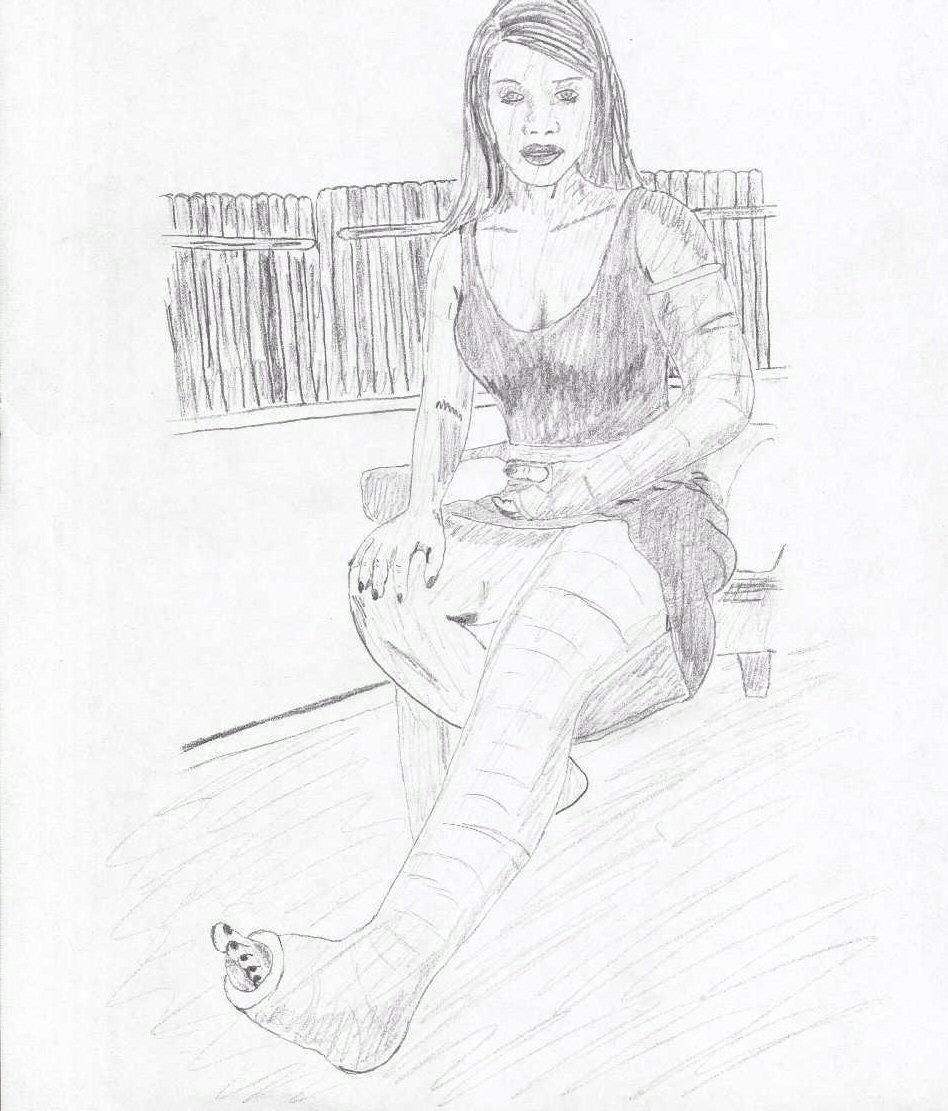
\includegraphics{images/kicks21.jpg}
\end{center}
